%% LaTeX2e Template by Stephen Iota (https://stepheniota.com/)
%% last updated: Feb. 2019
%% for papers
%\documentclass[aps,preprint,notitlepage]{revtex4-1}
%% https://www-d0.fnal.gov/Run2Physics/WWW/templates/revtex4.pdf
%% https://cdn.journals.aps.org/files/revtex/auguide4-1.pdf
%% ^^ revTeX4-1 class options

%% for other
\documentclass[11pt]{article}
\usepackage{geometry} % let's be honest, standard LaTeX margins are GaRbagE for most purposes
%%%%%%%%%%%%%%%%
%%% Packages %%%
%%%%%%%%%%%%%%%%

\usepackage[utf8]{inputenc}
\usepackage[noadjust]{cite}
\usepackage{lipsum}
\usepackage{amsmath}
\usepackage{amssymb}
\usepackage{amsfonts}
\usepackage{physics} %http://ftp.math.purdue.edu/mirrors/ctan.org/macros/latex/contrib/physics/physics.pdf
\usepackage[thinc]{esdiff} % easy derivatives
\usepackage{graphicx} % \includegraphics{ }
\usepackage[shortlabels]{enumitem} % change labels in enum/item environments
\usepackage[dvipsnames]{xcolor} % colored links=
%\usepackage{footmisc} % http://mirror.utexas.edu/ctan/macros/latex/contrib/footmisc/footmisc.pdf
%\usepackage[small]{titlesec} % [small,medium,big] << controls size of *section text
%\usepackage{fancyhdr} %http://tug.ctan.org/tex-archive/macros/latex/contrib/fancyhdr/fancyhdr.pdf
% always put this at the end
\usepackage[
	colorlinks=true,
	citecolor=NavyBlue!90!black,
	linkcolor=NavyBlue!75!black,
	urlcolor=green!50!black,
	hypertexnames=false]{hyperref}

 %%%%%%%%%%%%%%%%%%
 %% New Commands %%
 %%%%%%%%%%%%%%%%%%
\newcommand{\email}[1]{\texttt{\href{mailto:#1}{#1}}}


%%%%%%%%%%%%%%%%%%
%% Front Matter %%
%%%%%%%%%%%%%%%%%%

%\pagenumbering{gobble} % no page numbers
\graphicspath{{figures/}} % set directory for figures
%\setcounter{section}{-1} % start with section 0


%%%%%%%%%%%%%
%%% Title %%%
%%%%%%%%%%%%%
\begin{document}

\begin{center}

\Large{\textsc{PSet 2}: \textbf{Fluids}}
\end{center}
\vspace{.5mm}


%%%%%%%%%%
%% INFO %%
%%%%%%%%%%

\begin{tabular}{rl}
\textsc{SI Leader}:
&
Stephen Iota (\email{siota001@ucr.edu})
\\
\textsc{Course}:
&
Physics 40B (Spring 2019), Prof.~Barsukov
\\
\textsc{Date}:
&
\today
\end{tabular}

%%%%%%%%%%%%%%
%% PROBLEMS %%
%%%%%%%%%%%%%%


\section{Pressure and velocity relationship}


Gas flows through the pipe of the figure below. You can't see into the pipe to know how the inner diameter changes. Rank in order, from largest to smallest, the gas speeds $v_a$, $v_b$, and $v_c$ at points $a$, $b$, and $c$. Explain.

\begin{figure}[h!]
	\centering
	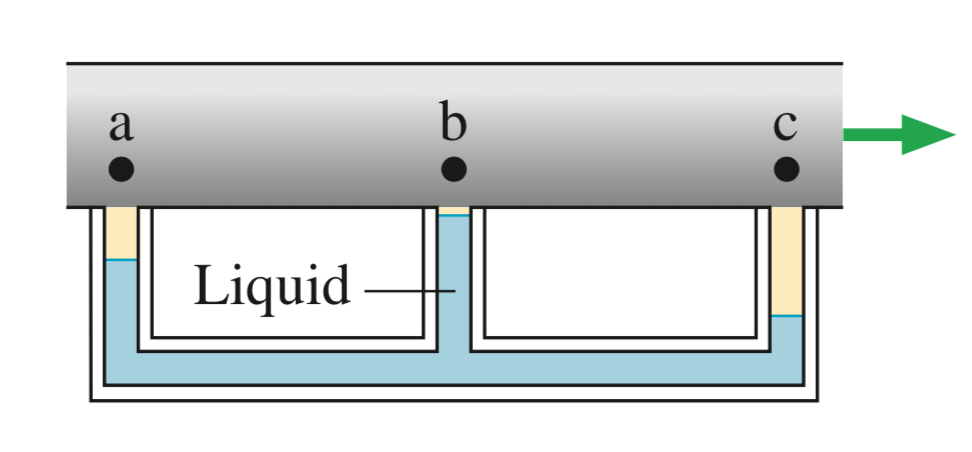
\includegraphics[width=0.5\linewidth]{pset2_fig2}
	\caption{Gas pipe \label{gas}}
	\end{figure}




\section{Bernoulli's principle}
Show that Bernoulli's principle is just another statement of conservation of energy. \\
Hint: What is the relationship between force and energy?


\section{Hydraulic lift}
Derive the equation for the hydraulic lift.


\section{Fluid dynamics}
\begin{enumerate}[(i)]


\item A 1.0-cm-diameter pipe widens to 2.0 cm, then narrows to 5.0 mm. Liquid flows through the first segment at a speed of 4.0 m/s.
\begin{enumerate}[(a)]
	\item What is the speed through the second and third segments?
	\item What is the volume flow rate through the pipe? 
\end{enumerate}

\newpage
\item What does the top pressure gauge read in the figure below?



\begin{figure}[h!]
	\centering
	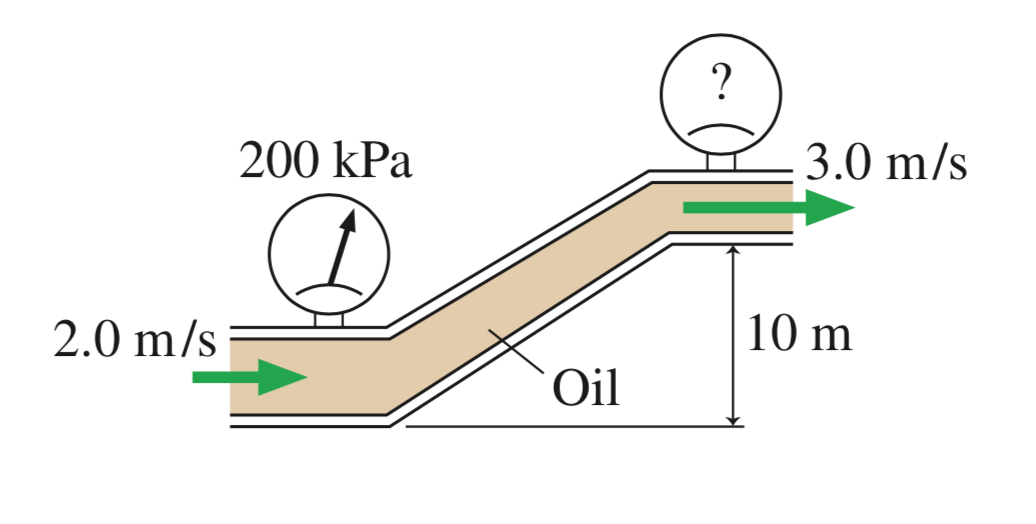
\includegraphics[width=0.5\linewidth]{pset2_fig1}
	\end{figure}


\end{enumerate}


\end{document}
